% Figure 2 of "Galashin's Conjecture 4.3 via a convex gradient": the half-open reading lemma on the
% resolved boundary, cut open for n = 8. Source of clh_halfopen_arcs.pdf, typeset in the paper's own
% fonts (T1, Latin Modern, 11pt) at the paper's text width (6.5in), so \includegraphics does not
% rescale it. Build from this directory:
%   pdflatex clh_halfopen_arcs.tex && pdftocairo -svg clh_halfopen_arcs.pdf clh_halfopen_arcs.svg
\documentclass[11pt]{standalone}
\usepackage[T1]{fontenc}
\usepackage{lmodern}
\usepackage{amsmath,amssymb}
\usepackage{tikz}
\usetikzlibrary{arrows.meta}

% the palette of the paper's other figures: blue solid for the arc of p, ochre dashed for that of q
\definecolor{ink}{HTML}{233740}
\definecolor{muted}{HTML}{65757D}
\definecolor{pblue}{HTML}{0072B2}
\definecolor{qochre}{HTML}{B87827}
\definecolor{sharebg}{HTML}{ECE7F5}
\definecolor{shadeline}{HTML}{8E7CC3}

% x-positions of the refined points j^- (exit) and j^+ (entry); the cut-open circle runs from 0 to \xend
\newcommand{\xm}[1]{\fpeval{0.5+(#1-1)*1.08}}
\newcommand{\xp}[1]{\fpeval{0.5+(#1-1)*1.08+0.4}}
\newcommand{\xend}{8.96}
\newcommand{\lo}{0.3}  % height of the lower arc above the line
\newcommand{\hi}{0.66}  % height of the upper arc

\tikzset{
  base/.style={draw=muted, line width=0.5pt},
  exit/.style={circle, draw=ink, fill=white, line width=0.6pt, inner sep=0pt, minimum size=4.6pt},
  entry/.style={circle, draw=ink, fill=ink, line width=0.6pt, inner sep=0pt, minimum size=4.6pt},
  arcP/.style={pblue, line width=1.4pt},
  arcQ/.style={qochre, line width=1.4pt, dash pattern=on 4pt off 1.6pt},
  open end/.style={{Parenthesis[length=3.4pt,width=9pt]}-},
  closed end/.style={-{Bracket[length=1.6pt,width=9pt]}},
  both ends/.style={{Parenthesis[length=3.4pt,width=9pt]}-{Bracket[length=1.6pt,width=9pt]}},
  lab/.style={font=\footnotesize, inner sep=1.2pt},
}

% \refinedline{y}: the cut-open boundary with its 2n refined points and integer labels
\newcommand{\refinedline}[1]{%
  \draw[base] (0,#1) -- (\xend,#1);
  \draw[base] (0,#1-0.1) -- (0,#1+0.1);
  \draw[base] (\xend,#1-0.1) -- (\xend,#1+0.1);
  \foreach \j in {1,...,8} {
    \node[exit]  at (\xm{\j},#1) {};
    \node[entry] at (\xp{\j},#1) {};
    \node[font=\footnotesize, text=muted] at ({(\xm{\j}+\xp{\j})/2},#1-0.36) {$\j$};
  }
}
% \sharedbox{j}{y}: the integer j shared by an exit and an entry
\newcommand{\sharedbox}[2]{%
  \fill[sharebg, draw=shadeline, line width=0.4pt, rounded corners=2.5pt]
    ({\xm{#1}-0.17},#2-0.17) rectangle ({\xp{#1}+0.17},#2+0.17);
}
% \arcbar{style}{u}{v}{y}{h}{label u}{label v}: the refined arc J(u^+,v^-) at height h above the line
% at y, open at the entry u^+ and closed at the exit v^-; it passes the cut when v <= u. The style is
% arcP or arcQ, and the labels take its colour.
\newcommand{\arcbar}[7]{%
  \pgfmathsetmacro{\xa}{\xp{#2}}\pgfmathsetmacro{\xb}{\xm{#3}}
  \ifdim\xa pt<\xb pt
    \draw[#1, both ends] (\xa,#4+#5) -- (\xb,#4+#5);
  \else
    \draw[#1, open end] (\xa,#4+#5) -- (\xend+0.14,#4+#5);
    \draw[#1, closed end] (-0.14,#4+#5) -- (\xb,#4+#5);
  \fi
  \node[lab, anchor=east, #1, solid] at (\xa-0.05,#4+#5+0.03) {#6};
  \node[lab, anchor=west, #1, solid] at (\xb+0.05,#4+#5+0.03) {#7};
}
\newcommand{\paneltitle}[2]{\node[anchor=base west, font=\small, text=ink, inner sep=0pt] at (0,#1) {#2};}
\newcommand{\panelnote}[2]{%
  \node[anchor=north west, text width=6.75cm, font=\footnotesize, text=ink, inner sep=0pt,
        align=flush left] at (9.5,#1) {#2};}

\begin{document}
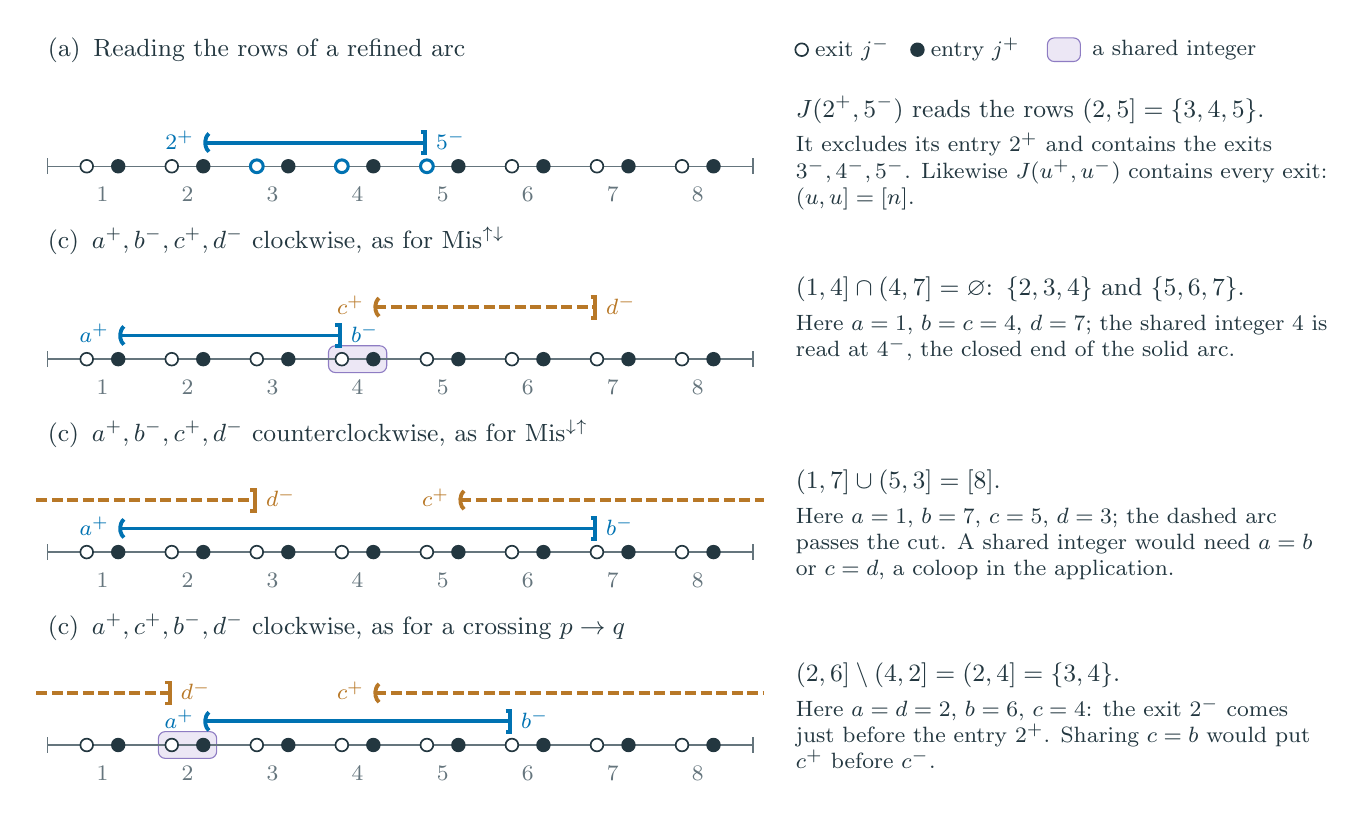
\begin{tikzpicture}[x=1cm,y=1cm]
\useasboundingbox (-0.25,-9.33) rectangle (16.26,0.36);

% legend, top right
\begin{scope}[shift={(9.5,0.08)}]
  \node[exit] at (0.08,0) {};
  \node[lab, anchor=west, text=ink] at (0.2,0) {exit $j^-$};
  \node[entry] at (1.55,0) {};
  \node[lab, anchor=west, text=ink] at (1.67,0) {entry $j^+$};
  \fill[sharebg, draw=shadeline, line width=0.4pt, rounded corners=2.5pt] (3.2,-0.15) rectangle (3.62,0.15);
  \node[lab, anchor=west, text=ink] at (3.72,0) {a shared integer};
\end{scope}

% ---------------------------------------------------------------- (a) the reading
\paneltitle{0}{(a)\enspace Reading the rows of a refined arc}
\refinedline{-1.4}
\arcbar{arcP}{2}{5}{-1.4}{\lo}{$2^+$}{$5^-$}
\foreach \j in {3,4,5} \node[exit, draw=pblue, line width=1.1pt] at (\xm{\j},-1.4) {};
\panelnote{-0.5}{%
  {\small $J(2^+,5^-)$ reads the rows $(2,5]=\{3,4,5\}$.}\\[3pt]
  It excludes its entry $2^+$ and contains the exits $3^-,4^-,5^-$. Likewise $J(u^+,u^-)$
  contains every exit: $(u,u]=[n]$.}

% ---------------------------------------------------------------- (L1)
\paneltitle{-2.45}{(c)\enspace $a^+,b^-,c^+,d^-$ clockwise, as for $\mathrm{Mis}^{\uparrow\downarrow}$}
\sharedbox{4}{-3.85}
\refinedline{-3.85}
\arcbar{arcP}{1}{4}{-3.85}{\lo}{$a^+$}{$b^-$}
\arcbar{arcQ}{4}{7}{-3.85}{\hi}{$c^+$}{$d^-$}
\panelnote{-2.8}{%
  {\small $(1,4]\cap(4,7]=\varnothing$:\enspace $\{2,3,4\}$ and $\{5,6,7\}$.}\\[3pt]
  Here $a=1$, $b=c=4$, $d=7$; the shared integer $4$ is read at $4^-$, the closed end of the
  solid arc.}

% ---------------------------------------------------------------- (L2)
\paneltitle{-4.9}{(c)\enspace $a^+,b^-,c^+,d^-$ counterclockwise, as for $\mathrm{Mis}^{\downarrow\uparrow}$}
\refinedline{-6.3}
\arcbar{arcP}{1}{7}{-6.3}{\lo}{$a^+$}{$b^-$}
\arcbar{arcQ}{5}{3}{-6.3}{\hi}{$c^+$}{$d^-$}
\panelnote{-5.25}{%
  {\small $(1,7]\cup(5,3]=[8]$.}\\[3pt]
  Here $a=1$, $b=7$, $c=5$, $d=3$; the dashed arc passes the cut. A shared integer would need $a=b$
  or $c=d$, a coloop in the application.}

% ---------------------------------------------------------------- (L3)
\paneltitle{-7.35}{(c)\enspace $a^+,c^+,b^-,d^-$ clockwise, as for a crossing $p\to q$}
\sharedbox{2}{-8.75}
\refinedline{-8.75}
\arcbar{arcP}{2}{6}{-8.75}{\lo}{$a^+$}{$b^-$}
\arcbar{arcQ}{4}{2}{-8.75}{\hi}{$c^+$}{$d^-$}
\panelnote{-7.7}{%
  {\small $(2,6]\setminus(4,2]=(2,4]=\{3,4\}$.}\\[3pt]
  Here $a=d=2$, $b=6$, $c=4$: the exit $2^-$ comes just before the entry $2^+$. Sharing $c=b$
  would put $c^+$ before $c^-$.}
\end{tikzpicture}
\end{document}
